\documentclass{beamer}
\usepackage{amsmath,graphics}
\usepackage{amssymb}

\usetheme{default}
\usepackage{xcolor}

\definecolor{solarizedBase03}{HTML}{002B36}
\definecolor{solarizedBase02}{HTML}{073642}
\definecolor{solarizedBase01}{HTML}{586e75}
\definecolor{solarizedBase00}{HTML}{657b83}
\definecolor{solarizedBase0}{HTML}{839496}
\definecolor{solarizedBase1}{HTML}{93a1a1}
\definecolor{solarizedBase2}{HTML}{EEE8D5}
\definecolor{solarizedBase3}{HTML}{FDF6E3}
\definecolor{solarizedYellow}{HTML}{B58900}
\definecolor{solarizedOrange}{HTML}{CB4B16}
\definecolor{solarizedRed}{HTML}{DC322F}
\definecolor{solarizedMagenta}{HTML}{D33682}
\definecolor{solarizedViolet}{HTML}{6C71C4}
%\definecolor{solarizedBlue}{HTML}{268BD2}
\definecolor{solarizedBlue}{HTML}{134676}
\definecolor{solarizedCyan}{HTML}{2AA198}
\definecolor{solarizedGreen}{HTML}{859900}
\definecolor{myBlue}{HTML}{162DB0}%{261CA4}
\setbeamercolor*{item}{fg=myBlue}
\setbeamercolor{normal text}{fg=solarizedBase03, bg=solarizedBase3}
\setbeamercolor{alerted text}{fg=myBlue}
\setbeamercolor{example text}{fg=myBlue, bg=solarizedBase3}
\setbeamercolor*{frametitle}{fg=solarizedRed}
\setbeamercolor*{title}{fg=solarizedRed}
\setbeamercolor{block title}{fg=myBlue, bg=solarizedBase3}
\setbeameroption{hide notes}
\setbeamertemplate{note page}[plain]
\beamertemplatenavigationsymbolsempty
\usefonttheme{professionalfonts}
\usefonttheme{serif}

\usepackage{fourier}

\def\vec#1{\mathchoice{\mbox{\boldmath$\displaystyle#1$}}
{\mbox{\boldmath$\textstyle#1$}}
{\mbox{\boldmath$\scriptstyle#1$}}
{\mbox{\boldmath$\scriptscriptstyle#1$}}}
\definecolor{OwnGrey}{rgb}{0.560,0.000,0.000} % #999999
\definecolor{OwnBlue}{rgb}{0.121,0.398,0.711} % #1f64b0
\definecolor{red4}{rgb}{0.5,0,0}
\definecolor{blue4}{rgb}{0,0,0.5}
\definecolor{Blue}{rgb}{0,0,0.66}
\definecolor{LightBlue}{rgb}{0.9,0.9,1}
\definecolor{Green}{rgb}{0,0.5,0}
\definecolor{LightGreen}{rgb}{0.9,1,0.9}
\definecolor{Red}{rgb}{0.9,0,0}
\definecolor{LightRed}{rgb}{1,0.9,0.9}
\definecolor{White}{gray}{1}
\definecolor{Black}{gray}{0}
\definecolor{LightGray}{gray}{0.8}
\definecolor{Orange}{rgb}{0.1,0.2,1}
\setbeamerfont{sidebar right}{size=\scriptsize}
\setbeamercolor{sidebar right}{fg=Black}

\renewcommand{\emph}[1]{{\textcolor{solarizedRed}{\itshape #1}}}

\newcommand\cA{\mathcal A}
\newcommand\cB{\mathcal B}
\newcommand\cC{\mathcal C}
\newcommand\cD{\mathcal D}
\newcommand\cE{\mathcal E}
\newcommand\cF{\mathcal F}
\newcommand\cG{\mathcal G}
\newcommand\cH{\mathcal H}
\newcommand\cI{\mathcal I}
\newcommand\cJ{\mathcal J}
\newcommand\cK{\mathcal K}
\newcommand\cL{\mathcal L}
\newcommand\cM{\mathcal M}
\newcommand\cN{\mathcal N}
\newcommand\cO{\mathcal O}
\newcommand\cP{\mathcal P}
\newcommand\cQ{\mathcal Q}
\newcommand\cR{\mathcal R}
\newcommand\cS{\mathcal S}
\newcommand\cT{\mathcal T}
\newcommand\cU{\mathcal U}
\newcommand\cV{\mathcal V}
\newcommand\cW{\mathcal W}
\newcommand\cX{\mathcal X}
\newcommand\cY{\mathcal Y}
\newcommand\cZ{\mathcal Z}

\newcommand\fA{\mathfrak A}
\newcommand\fB{\mathfrak B}
\newcommand\fC{\mathfrak C}
\newcommand\fD{\mathfrak D}
\newcommand\fE{\mathfrak E}
\newcommand\fF{\mathfrak F}
\newcommand\fG{\mathfrak G}
\newcommand\fH{\mathfrak H}
\newcommand\fI{\mathfrak I}
\newcommand\fJ{\mathfrak J}
\newcommand\fK{\mathfrak K}
\newcommand\fL{\mathfrak L}
\newcommand\fM{\mathfrak M}
\newcommand\fN{\mathfrak N}
\newcommand\fO{\mathfrak O}
\newcommand\fP{\mathfrak P}
\newcommand\fQ{\mathfrak Q}
\newcommand\fR{\mathfrak R}
\newcommand\fS{\mathfrak S}
\newcommand\fT{\mathfrak T}
\newcommand\fU{\mathfrak U}
\newcommand\fV{\mathfrak V}
\newcommand\fW{\mathfrak W}
\newcommand\fX{\mathfrak X}
\newcommand\fY{\mathfrak Y}
\newcommand\fZ{\mathfrak Z}

\newcommand\fa{\mathfrak a}
\newcommand\fb{\mathfrak b}
\newcommand\fc{\mathfrak c}
\newcommand\fd{\mathfrak d}
\newcommand\fe{\mathfrak e}
\newcommand\ff{\mathfrak f}
\newcommand\fg{\mathfrak g}
\newcommand\fh{\mathfrak h}
%\newcommand\fi{\mathfrak i}
\newcommand\fj{\mathfrak j}
\newcommand\fk{\mathfrak k}
\newcommand\fl{\mathfrak l}
\newcommand\fm{\mathfrak m}
\newcommand\fn{\mathfrak n}
\newcommand\fo{\mathfrak o}
\newcommand\fp{\mathfrak p}
\newcommand\fq{\mathfrak q}
\newcommand\fr{\mathfrak r}
\newcommand\fs{\mathfrak s}
\newcommand\ft{\mathfrak t}
\newcommand\fu{\mathfrak u}
\newcommand\fv{\mathfrak v}
\newcommand\fw{\mathfrak w}
\newcommand\fx{\mathfrak x}
\newcommand\fy{\mathfrak y}
\newcommand\fz{\mathfrak z}

\newcommand\vA{\vec A}
\newcommand\vB{\vec B}
\newcommand\vC{\vec C}
\newcommand\vD{\vec D}
\newcommand\vE{\vec E}
\newcommand\vF{\vec F}
\newcommand\vG{\vec G}
\newcommand\vH{\vec H}
\newcommand\vI{\vec I}
\newcommand\vJ{\vec J}
\newcommand\vK{\vec K}
\newcommand\vL{\vec L}
\newcommand\vM{\vec M}
\newcommand\vN{\vec N}
\newcommand\vO{\vec O}
\newcommand\vP{\vec P}
\newcommand\vQ{\vec Q}
\newcommand\vR{\vec R}
\newcommand\vS{\vec S}
\newcommand\vT{\vec T}
\newcommand\vU{\vec U}
\newcommand\vV{\vec V}
\newcommand\vW{\vec W}
\newcommand\vX{\vec X}
\newcommand\vY{\vec Y}
\newcommand\vZ{\vec Z}

\newcommand\va{\vec a}
\newcommand\vb{\vec b}
\newcommand\vc{\vec c}
\newcommand\vd{\vec d}
\newcommand\ve{\vec e}
\newcommand\vf{\vec f}
\newcommand\vg{\vec g}
\newcommand\vh{\vec h}
\newcommand\vi{\vec i}
\newcommand\vj{\vec j}
\newcommand\vk{\vec k}
\newcommand\vl{\vec l}
\newcommand\vm{\vec m}
\newcommand\vn{\vec n}
\newcommand\vo{\vec o}
\newcommand\vp{\vec p}
\newcommand\vq{\vec q}
\newcommand\vr{\vec r}
\newcommand\vs{\vec s}
\newcommand\vt{\vec t}
\newcommand\vu{\vec u}
\newcommand\vv{\vec v}
\newcommand\vw{\vec w}
\newcommand\vx{\vec x}
\newcommand\vy{\vec y}
\newcommand\vz{\vec z}

\renewcommand\AA{\mathbb A}
\newcommand\NN{\mathbb N}
\newcommand\ZZ{\mathbb Z}
\newcommand\PP{\mathbb P}
\newcommand\QQ{\mathbb Q}
\newcommand\RR{\mathbb R}
\renewcommand\SS{\mathbb S}
\newcommand\CC{\mathbb C}

\newcommand{\ord}{\mathrm{ord}}
\newcommand{\id}{\mathrm{id}}
\newcommand{\pr}{\mathrm{P}}
\newcommand{\Vol}{\mathrm{vol}}
\newcommand\norm[1]{\left\|{#1}\right\|} 
\newcommand\sign{\mathrm{sign}}
\newcommand{\eps}{\varepsilon}
\newcommand{\abs}[1]{\left|#1\right|}
\newcommand\bc[1]{\left({#1}\right)} 
\newcommand\cbc[1]{\left\{{#1}\right\}} 
\newcommand\bcfr[2]{\bc{\frac{#1}{#2}}} 
\newcommand{\bck}[1]{\left\langle{#1}\right\rangle} 
\newcommand\brk[1]{\left\lbrack{#1}\right\rbrack} 
\newcommand\scal[2]{\bck{{#1},{#2}}} 
\newcommand{\vecone}{\mathbb{1}}
\newcommand{\tensor}{\otimes}
\newcommand{\diag}{\mathrm{diag}}
\newcommand{\ggt}{\mathrm{ggT}}
\newcommand{\kgv}{\mathrm{kgV}}
\newcommand{\trans}{\top}

\newcommand{\Karonski}{Karo\'nski}
\newcommand{\Erdos}{Erd\H{o}s}
\newcommand{\Renyi}{R\'enyi}
\newcommand{\Lovasz}{Lov\'asz}
\newcommand{\Juhasz}{Juh\'asz}
\newcommand{\Bollobas}{Bollob\'as}
\newcommand{\Furedi}{F\"uredi}
\newcommand{\Komlos}{Koml\'os}
\newcommand{\Luczak}{\L uczak}
\newcommand{\Kucera}{Ku\v{c}era}
\newcommand{\Szemeredi}{Szemer\'edi}

\renewcommand{\ae}{\"a}
\renewcommand{\oe}{\"o}
\newcommand{\ue}{\"u}
\newcommand{\Ae}{\"A}
\newcommand{\Oe}{\"O}
\newcommand{\Ue}{\"U}

\newcommand{\mytitle}{Vektoren}

\title[Linadi]{\mytitle}
\author[Amin Coja-Oghlan]{Amin Coja-Oghlan}
\institute[Frankfurt]{JWGUFFM}
\date{}

\begin{document}

\frame[plain]{\titlepage}

\begin{frame}\frametitle{\mytitle}
	\begin{block}{Definition}
		Sei $n\in\NN$.
	\begin{itemize}
		\item Eine $n\times 1$-Matrix ist ein \emph{Spaltenvektor} der Gr\oe\ss e $n$.
		\item Eine $1\times n$-Matrix ist ein \emph{Zeilenvektor} der Gr\oe\ss e $n$.
		\item Wir identifizieren die Menge $\RR^n$ aller $n$-Tupel reeller Zahlen mit der Menge $\RR^{n\times 1}$ der Spaltenvektoren.
	\end{itemize}
	\end{block}
\end{frame}

\begin{frame}\frametitle{\mytitle}
	\begin{block}{Beispiel}
	\begin{itemize}
		\item $\begin{pmatrix}1\\2\\3\end{pmatrix}\in\RR^{3\times 1}=\RR^3$ ist ein Spaltenvektor der Gr\oe\ss e 3.
		\item $\begin{pmatrix}1&2&3\end{pmatrix}\in\RR^{1\times 3}$ ist ein Zeilenvektor der Gr\oe\ss e 3.
	\end{itemize}
	\end{block}
\end{frame}

\begin{frame}\frametitle{\mytitle}
	\begin{block}{Rechnen mit Vektoren}
	\begin{itemize}
		\item Weil Vektoren spezielle Matrizen sind, wissen wir schon, wie man sie addiert.
		\item Wir wissen auch, wie man sie mit Skalaren multipliziert.
	\end{itemize}
	\end{block}
\end{frame}

\begin{frame}\frametitle{\mytitle}
	\begin{block}{Beispiele}
	\begin{align*}
		\begin{pmatrix}1\\2\\3\end{pmatrix}+\begin{pmatrix}4\\5\\6\end{pmatrix}&=\begin{pmatrix}5\\7\\9\end{pmatrix}\\
		-2\cdot\begin{pmatrix}1\\2\\3\end{pmatrix}&=\begin{pmatrix}-2\\-4\\-6\end{pmatrix}\\
		\begin{pmatrix}1&2&3\end{pmatrix}+\begin{pmatrix}4&5&6\end{pmatrix}&=\begin{pmatrix}5&7&9\end{pmatrix}\\
		-2\cdot\begin{pmatrix}1&2&3\end{pmatrix}&=\begin{pmatrix}-2&-4&-6\end{pmatrix}
	\end{align*}
	\end{block}
\end{frame}

\begin{frame}\frametitle{\mytitle}
	\begin{block}{Geometrische Interpretation}
	\begin{itemize}
		\item Vektoren der Gr\oe\ss e 2 k\oe nnen wir als Punkte in der Ebene interpretieren.
		\item Den ersten Eintrag des Vektors interpretieren wir als seine $x$-Koordinate.
		\item Den zweiten Eintrag des Vektors interpretieren wir als seine $y$-Koordinate.
	\end{itemize}
	\end{block}
\end{frame}

\begin{frame}\frametitle{\mytitle}
	\hfill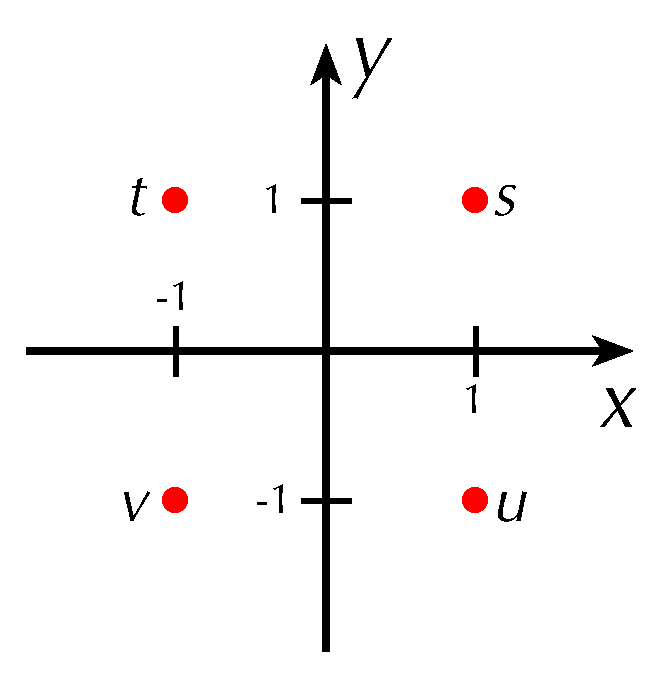
\includegraphics[height=50mm]{pics/vectors.pdf}
	\begin{block}{Beispiel}
		Die Vektoren $s=\binom11$, $t=\binom{-1}1$, $u=\binom1{-1}$, $v=\binom{-1}{-1}$.
	\end{block}
\end{frame}

\begin{frame}\frametitle{\mytitle}
	\begin{block}{Geometrische Interpretation}
	\begin{itemize}
		\item Vektoren der Gr\oe\ss e 3 k\oe nnen wir als Punkte im Raum interpretiert werden.
		\item Zur $x$- und $y$-Achse kommt dann die $z$-Achse hinzu.
		\item Gr\oe\ss ere Vektoren haben keine einfache anschauliche Interpretation.
	\end{itemize}
	\end{block}
\end{frame}

\begin{frame}\frametitle{\mytitle}
	\begin{block}{Geometrische Interpretation: Skalierung}
	\begin{itemize}
		\item F\ue r einen Vektor $u$ und eine Zahl $c>0$ k\oe nnen wir uns den Vektor $c\cdot u$ als eine Skalierung von $u$ vorstellen.
		\item Wenn $c>1$, wird der Vektor gestreckt.
		\item Wenn $c<1$, wird der Vektor gestaucht.
	\end{itemize}
	\end{block}
\end{frame}

\begin{frame}\frametitle{\mytitle}
	\begin{block}{Geometrische Interpretation: Skalierung}
	\begin{itemize}
		\item F\ue r einen Vektor $u$ wir uns $-u$ als eine Reflektion von $u$ am Nullpunkt vorstellen.
		\item Entsprechent ist $c\cdot u$ f\ue r $c<0$ eine Reflektion gefolgt von einer Streckung oder Stauchung.
	\end{itemize}
	\end{block}
\end{frame}

\begin{frame}\frametitle{\mytitle}
	\hfill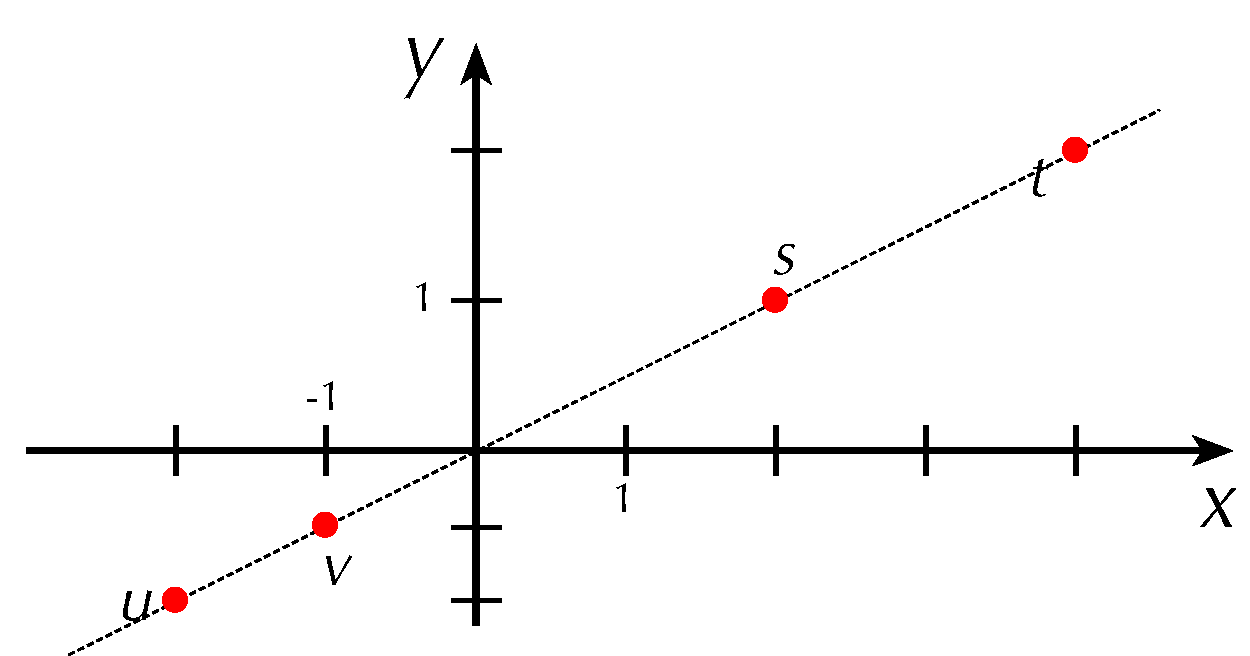
\includegraphics[height=40mm]{pics/vectorscaling.pdf}
	\begin{block}{Beispiele}
		Es sei $s=\binom21$.
		\begin{itemize}
			\item $t=2\cdot s=\binom42$ ist der aufs Doppelte gestreckte Vektor.
			\item $u=-s=\binom{-2}{-1}$ ist die Reflektion durch den Nullpunkt.
			\item $v=-\frac12s=\binom{-1}{-1/2}$ ist die auf die H\ae lfte gestauchte Reflektion. 
			\item Die Menge $\{c\cdot s:c\in\RR\}$ bildet die gestrichelte Gerade.
		\end{itemize}
	\end{block}
\end{frame}

\begin{frame}\frametitle{\mytitle}
	\hfill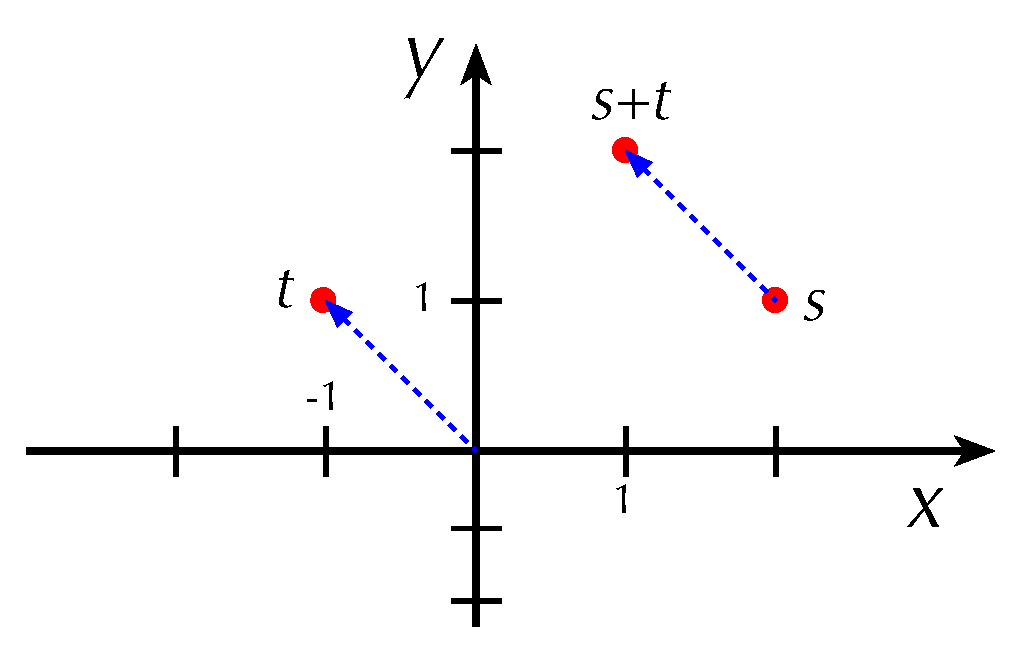
\includegraphics[height=50mm]{pics/vectoradd.pdf}
	\begin{block}{Geometrische Interpretation: Verschiebung}
	\begin{itemize}
	\item Wenn $s,t$ Vektoren sind, k\oe nnen wir uns $s+t$ als die Verschiebung von $t$ zu $s$ vorstellen.
	\item \emph{Beispiel:} $s=\binom 21$, $t=\binom{-1}1$, $s+t=\binom12$
	\end{itemize}
	\end{block}
\end{frame}

\begin{frame}\frametitle{\mytitle}
	\begin{block}{Das Skalarprodukt}
		\begin{itemize}
			\item Seien $u=(u_i)_{i=1,\ldots,n},v=(v_i)_{i=1,\ldots,n}\in\RR^n$ Vektoren.
			\item Das \emph{Skalarprodukt} von $u,v$ ist definiert als
				\begin{align*}
					u^\trans v=\sum_{i=1}^nu_iv_i\in\RR.
				\end{align*}
			\item \emph{Beachte:} $u^\trans\in\RR^{1\times n}$ ist ein Zeilenvektor, so da\ss\ die Multiplikation auf der linken Seite ein Spezialfall der Matrixmultiplikation ist.
		\end{itemize}
	\end{block}
\end{frame}

\begin{frame}\frametitle{\mytitle}
	\begin{block}{Rechenregeln f\ue r das Skalarprodukt}
		\begin{description}
			\item[Kommutativit\ae t:] $u^\trans v=v^\trans u$
			\item[Linearit\ae t:] f\ue r alle $u,v,w\in\RR^n$ und $c\in\RR$ gilt
				\begin{align*}
					(u+v)^\trans w&=u^\trans w+v^\trans w\\
					(c\cdot u)^\trans w&=c\cdot(u^\trans w)
				\end{align*}
		\end{description}
	\end{block}
\end{frame}

\begin{frame}\frametitle{\mytitle}
	\begin{block}{Beispiele}
		\begin{align*}
			\binom12^\trans\cdot\binom34&=(1\ 2)\cdot\binom 34=1\cdot 3+2\cdot 4=11\\
			\begin{pmatrix}1\\-1\\0\end{pmatrix}^\trans\cdot\begin{pmatrix}0\\-1\\1\end{pmatrix}&=
			\begin{pmatrix}1&-1&0\end{pmatrix}\cdot\begin{pmatrix}0\\-1\\1\end{pmatrix}=1\cdot 0+(-1)\cdot(-1)+0\cdot 1=1
		\end{align*}
	\end{block}
\end{frame}

\begin{frame}\frametitle{\mytitle}
	\begin{block}{Definition}
		Die \emph{Norm} eines Vektors $u=(u_i)_i\in\RR^n$ ist definiert als
		\begin{align*}
			\|u\|&=\sqrt{u^\trans u}=\sqrt{\sum_{i=1}^nu_i^2}
		\end{align*}
		Wir nennen $u$ einen \emph{Einheitsvektor}, falls $\|u\|=1$.
	\end{block}
\end{frame}

\begin{frame}\frametitle{\mytitle}
	\hfill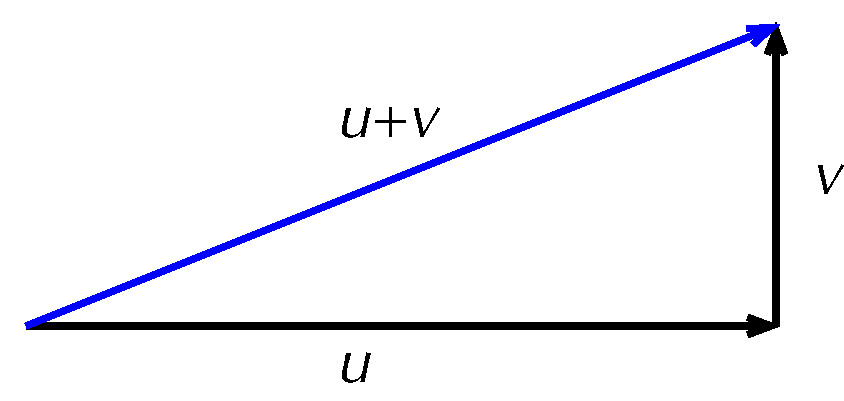
\includegraphics[height=30mm]{pics/triangleineq.pdf}
	\begin{block}{Rechenregeln f\ue r die Norm}
		F\ue r alle $u,v\in\RR^n$ und alle $c\in\RR$ gilt
	\begin{itemize}
		\item $\|0\|=0$
		\item $\|c\cdot u\|=|c|\cdot\|u\|$
		\item $\|u+v\|\leq\|u\|+\|v\|$ \hfill[``Dreiecksungleichung'']
	\end{itemize}
	\end{block}
\end{frame}

\begin{frame}\frametitle{\mytitle}
	\hfill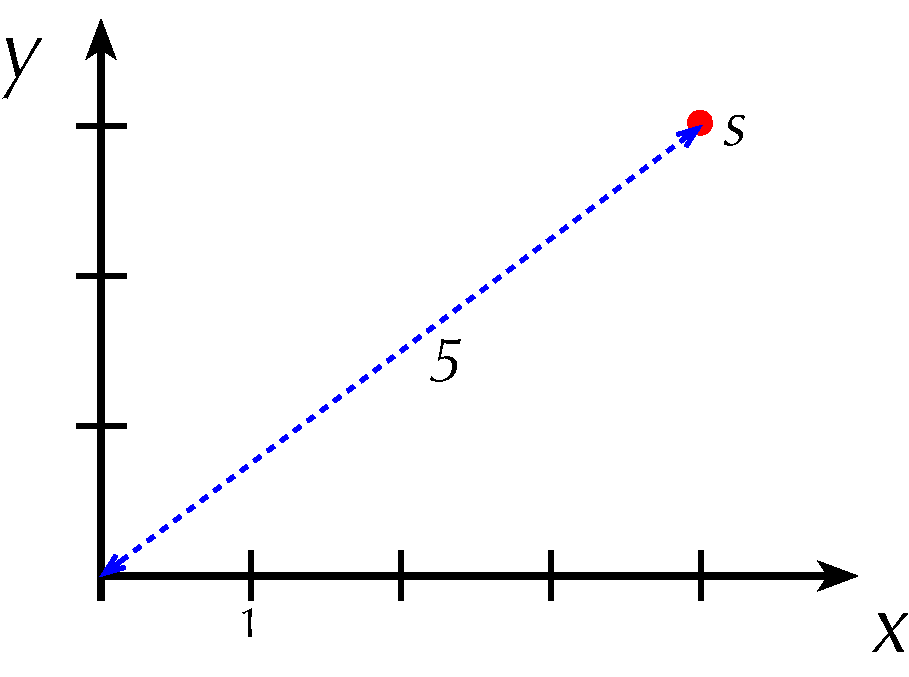
\includegraphics[height=40mm]{pics/vectornorm.pdf}
	\begin{block}{Geometrische Interpretation: Norm}
	\begin{itemize}
		\item Wir k\oe nnen uns die Norm als den Abstand des Vektors vom Nullpunkt vorstellen.
		\item \emph{Beispiel:} der Vektor $s=\binom 43$ hat Abstand $\sqrt{3^2+4^2}=5$ vom Nullpunkt.
	\end{itemize}
	\end{block}
\end{frame}

\begin{frame}\frametitle{\mytitle}
	\begin{block}{Definition}
		Der \emph{Winkel} zwischen zwei Vektoren $u,v\neq0$ ist definiert als
		\begin{align*}
			\angle(u,v)&=\arccos\bcfr{u^\trans v}{\|u\|\cdot\|v\|}
		\end{align*}
	\end{block}
\end{frame}

\begin{frame}\frametitle{\mytitle}
	\hfill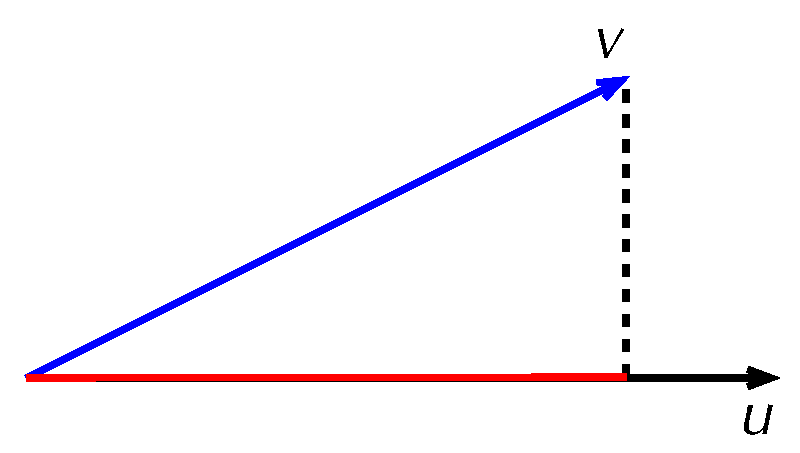
\includegraphics[height=30mm]{pics/scalarproduct.pdf}
	\begin{block}{Geometrische Interpretation: Skalarprodukt}
		\begin{itemize}
			\item $u^\trans v=\|u\|\cdot\|v\|\cdot\cos(\angle(u,v))$
			\item wenn $u$ ein Einheitsvektor ist, ist $|u^\trans v|$ die L\ae nge der Projektion von $v$ auf $u$
		\end{itemize}
	\end{block}
\end{frame}

\begin{frame}\frametitle{\mytitle}
	\begin{block}{Zusammenfassung}
		\begin{itemize}
			\item Addition von Vektoren und Multiplikation mit Skalaren sind Spezialf\ae lle der Matrixrechnung
			\item Die Norm mi\ss t die L\ae nge von Vektoren.
			\item Das Skalarprodukt kann aus den L\ae ngen und Winkeln zwischen zwei Vektoren bestimmt werden.
		\end{itemize}
	\end{block}
\end{frame}

\end{document}
